\documentclass[12pt, a4paper]{article}
\usepackage[utf8]{inputenc}
\usepackage[T1]{fontenc}
\usepackage[french]{babel}
\usepackage{geometry}
\usepackage{graphicx}
\usepackage{amsmath}
\usepackage{amssymb}
\usepackage{booktabs}
\usepackage{array}
\usepackage{enumitem}
\usepackage{xcolor}
\usepackage{ulem}
\usepackage{float}
\usepackage{caption}
\usepackage{adjustbox}
\usepackage{tikz}
\usepackage{enumitem}
\usepackage{fancyhdr} % Ajout du package pour les en-têtes

\usetikzlibrary{calc, shapes.geometric}
\geometry{margin=2cm}

% Configuration de l'en-tête
\pagestyle{fancy}
\fancyhf{} % Efface les en-têtes et pieds de page par défaut
\renewcommand{\headrulewidth}{0.4pt}
\renewcommand{\headrule}{\hrule width\headwidth height\headrulewidth}
\fancyhead[C]{\rule{\textwidth}{0.4pt}} % Ligne centrée
\fancyhead[R]{\textit{Investigation numérique}} % Texte à droite
\fancyfoot[C]{\thepage} % Numéro de page centré

% Marges réduites

\definecolor{blue1}{RGB}{0, 51, 102}
\definecolor{blue2}{RGB}{0, 102, 204}
\definecolor{gray1}{RGB}{240, 240, 240}

\geometry{margin=2.5cm}

\begin{document}
	\begin{titlepage}
		
		% Bordure autour de la page
		\begin{tikzpicture}[remember picture, overlay]
			\draw[line width=2pt, black] 
			($(current page.north west) + (0.5cm,-0.5cm)$) rectangle 
			($(current page.south east) + (-0.5cm,0.5cm)$);
		\end{tikzpicture}
		
		\centering
		
		% SOLUTION FONCTIONNELLE : Tableau avec alignement en bas
		\begin{tabular}{@{}p{0.25\textwidth}@{\hspace{2cm}}c@{\hspace{0.5cm}}p{0.5\textwidth}@{}}
			% Colonne de gauche (Français) - ALIGNÉ EN BAS
			\begin{minipage}[t][5cm][b]{0.39\textwidth}
				\raggedright
				\begin{center}
					{\small \textbf{RÉPUBLIQUE DU CAMEROUN}}\\
					{\small \textbf{******}}\\
					{\small \textbf{UNIVERSITÉ DE YAOUNDÉ}}\\
					{\small \textbf{I}}\\
					{\small \textbf{******}}\\
					{\small \textbf{ÉCOLE NATIONALE SUPÉRIEURE POLYTECHNIQUE}}\\
					{\small \textbf{******}}\\
					{\small \textbf{DÉPARTEMENT DU GÉNIE INFORMATIQUE}}\\
				\end{center}
			\end{minipage}
			&
			% Colonne du centre (LOGO EN BAS)
			\begin{minipage}[t][5cm][b]{0.2\textwidth}
				\centering
				
				\vspace*{\fill} % Pousse le logo vers le bas
				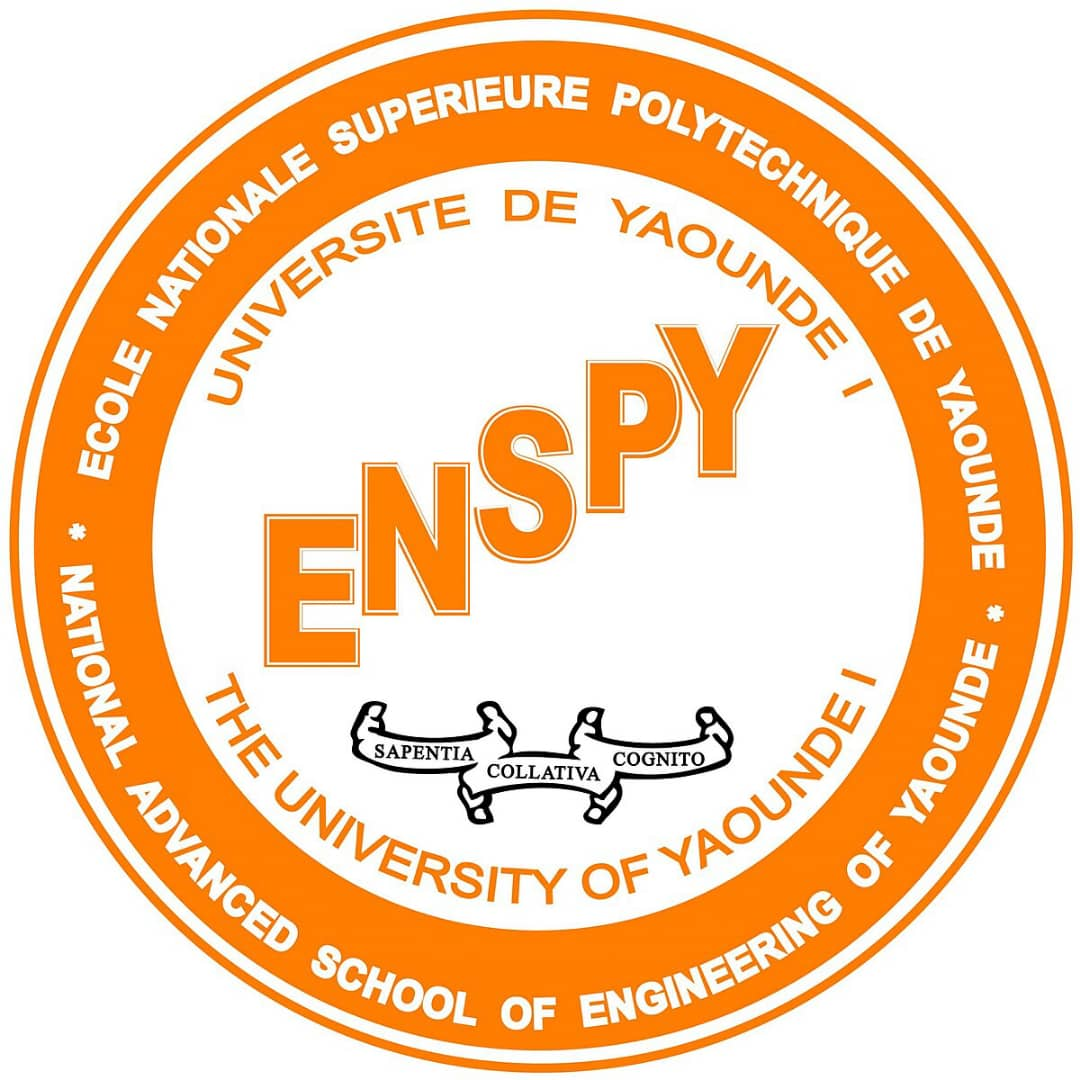
\includegraphics[width=\textwidth, height=3cm]{logo.jpeg}
				\vspace*{\fill} % Espace en bas
			\end{minipage}
			&
			% Colonne de droite (Anglais) - ALIGNÉ EN BAS
			\begin{minipage}[t][5cm][b]{0.36\textwidth}
				\raggedright
				\begin{center}
					{\small \textbf{REPUBLIC OF CAMEROON}}\\
					{\small \textbf{******}}\\
					{\small \textbf{UNIVERSITY OF YAOUNDE I}}\\
					{\small \textbf{******}}\\
					{\small \textbf{NATIONAL ADVANCED SCHOOL OF}}\\
					{\small \textbf{ENGINEERING}}\\
					{\small \textbf{******}}\\
					{\small \textbf{DEPARTMENT OF COMPUTER ENGINEERING}}\\
				\end{center}
			\end{minipage}
		\end{tabular}
		
		\vspace{1.5cm}
		
		% Ligne séparatrice
		\noindent\rule{0.9\textwidth}{0.8pt}\\
		\vspace{0.5cm}
		
		% Thème
		\vspace{0.8cm}
		{\Large \textbf{Synthese des exposés}}\\
		\vspace{0.8cm}
		
		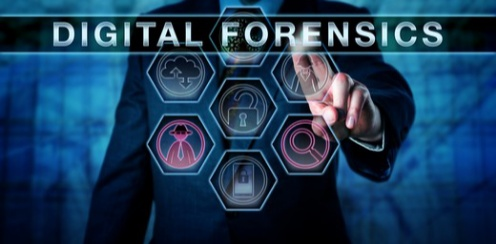
\includegraphics[width=0.5\textwidth]{For.jpeg}
		% Ligne séparatrice
		\noindent\rule{0.9\textwidth}{0.8pt}\\
		\vspace{1.5cm}
		
		% Informations étudiant
		\begin{tabular}{@{}>{\bfseries}l l@{}}
			\vspace{0.5cm}
			Réalisé par : & \textbf{NANTIA ZAGUE AXEL FRISKYL} \\
			\vspace{0.5cm}
			Matricule : & \textbf{22P105} \\
			\vspace{0.5cm}
			Spécialité : & \textbf{Cybersécurité et Investigation Numérique (CIN)} \\
			\vspace{0.5cm}
			UE : & \textbf{Introduction aux techniques de l'Investigations Numériques} \\
			\vspace{0.5cm}
			Sous la supervision de : & \textbf{Mr. MINKA MI NGUIDJOI Thierry Emmanuel} \\
			\vspace{0.5cm}
			Année académique : & \textbf{2025/2026} \\
		\end{tabular}
		
	\end{titlepage}
	
	% Page de garde sans en-tête
	\thispagestyle{empty}
	\newpage
	
	
	\title{\textbf{Resumer en blocs des exposés}}
	\author{}
	\date{}
	
	
	
	\maketitle
		
		\section{TROIS MEILLEURS OUTILS LOGICIELS DE RÉDACTION DE MÉMOIRE}
		
		La rédaction d'un mémoire est une entreprise complexe qui dépasse largement le cadre de la simple rédaction. Elle exige une gestion rigoureuse des sources, le respect des normes formelles et la structuration d'un contenu substantiel. Face à ce défi, j'ai analysé les outils logiciels disponibles et j'ai identifié trois catégories d'outils aux forces complémentaires, dont la synergie permet de créer un environnement de travail sur mesure. Aucune solution unique ne couvrant l'ensemble des besoins, c'est dans leur combinaison que réside la clé de l'efficacité.
		
		Ma première analyse porte sur les environnements de rédaction. J'ai examiné Overleaf, un éditeur LaTeX en ligne qui révolutionne l'approche académique. Sa philosophie repose sur l'accessibilité, la collaboration en temps réel et le maintien de standards professionnels. Il excelle par sa qualité typographique exceptionnelle, sa gestion avancée des références croisées et sa bibliothèque de modèles académiques. Cependant, je constate une courbe d'apprentissage significative, ce qui peut représenter un frein pour les non-initiés. En parallèle, j'ai évalué Microsoft Word, l'outil universel dont la prédominance s'explique par sa familiarité et sa compatibilité. Ses atouts majeurs pour un mémoire incluent la gestion avancée des styles pour structurer de longs documents, la génération automatique des tables et l'indispensable suivi des modifications pour les échanges avec le directeur. Je note toutefois ses limites, notamment une gestion bibliographique native basique et des risques d'instabilité sur des documents très volumineux. Au-delà de la rédaction, mon étude s'est concentrée sur un élément trop souvent sous-estimé : la gestion des références. C'est ici que Zotero s'impose comme un outil indispensable. Ce gestionnaire de références open-source centralise et organise l'ensemble des sources. Je suis particulièrement impressionné par sa capture automatique des métadonnées depuis les navigateurs web, son intégration transparente avec Word et Overleaf via des plugins dédiés, et son support de milliers de styles de citation académiques. Sa synchronisation cloud et son écosystème d'extensions en font un outil à la fois puissant et remarquablement flexible.
		
		Mon constat principal est que l'efficacité réelle de ces outils réside dans leur capacité à fonctionner en parfaite complémentarité. C'est pourquoi je propose plusieurs workflows optimisés, adaptés à des profils spécifiques. Pour un étudiant débutant ou en sciences humaines, je recommande le duo Word + Zotero. Cette combinaison offre le meilleur compromis : elle conserve l'environnement de rédaction familier de Word tout en compensant ses lacunes bibliographiques grâce au plugin Zotero, qui permet d'insérer des citations et de générer la bibliographie automatiquement. Pour les travaux exigeants des sciences exactes, où la précision typographique et la gestion des équations sont primordiales, je préconise la triade Overleaf + Zotero. Zotero gère la bibliographie, l'export BibTeX permet une intégration parfaite dans Overleaf, et ce dernier assure un rendu professionnel irréprochable. Enfin, pour les mémoires en co-direction ou les thèses, j'estime que l'association Overleaf + Zotero Groups est idéale. Elle crée un écosystème collaboratif parfaitement synchronisé, où Zotero Groups gère une bibliothèque de sources partagée tandis qu'Overleaf permet la rédaction en temps réel à plusieurs.
		
		En conclusion, cette analyse approfondie me permet d'affirmer que le choix des outils n'est pas anodin. Il doit être guidé par la nature du travail, le profil de l'étudiant et les impératifs de collaboration. Si je recommande chaudement la combinaison Overleaf et Zotero pour son excellence académique, je reste convaincu que ces outils, aussi sophistiqués soient-ils, ne sont que des instruments. La plus belle mise en page et la bibliographie la plus impeccable ne sauraient compenser un contenu faible. L'étudiant averti saura donc trouver le juste équilibre entre la maîtrise de l'outil, qui libère des contraintes techniques, et la profondeur de la recherche, qui demeure le véritable cœur du travail intellectuel.
		
		\section{CONCEPTION ET ANALYSE D'UN FAUX PROFIL TIKTOK}
		
		Ce projet pédagogique d'investigation numérique a permis d'explorer les mécanismes d'influence et d'engagement sur les réseaux sociaux à travers la création méthodique d'un faux profil TikTok dédié à la cybersécurité. La démarche adoptée a su allier rigueur technique et considérations éthiques, en utilisant des outils adaptés comme les services de messagerie temporaire pour préserver l'anonymat et les analyseurs de statistiques intégrés à la plateforme pour mesurer l'impact des publications. Le choix de la niche cybersécurité s'est révélé stratégique, permettant d'aborder des sujets sensibles tout en maintenant une finalité éducative et préventive. La conception des contenus - alliant visuels percutants, ton humoristique et messages clairs - a démontré l'importance d'une approche adaptée au public cible pour maximiser l'engagement sans sacrifier la valeur informative.
		
		L'analyse des résultats a mis en évidence l'efficacité de cette stratégie, avec des taux d'interaction significatifs sur l'ensemble des publications thématiques. Les contenus traitant des mots de passe, des risques du Wi-Fi public et des arnaques de phishing ont particulièrement resonné auprès de l'audience, générant des centaines de vues et de multiples interactions. Cette réception positive confirme l'actualité et l'importance des sujets abordés, tout en validant l'approche pédagogique choisie. Cependant, l'expérience a également révélé la fragilité de la frontière entre sensibilisation légitime et manipulation potentielle, soulignant la nécessité impérative d'un cadre éthique strict pour ce type d'exercice.
		
		Les enseignements tirés de cette investigation soulèvent des questions fondamentales sur l'usage des faux profils dans un contexte pédagogique. Si l'outil s'est avéré efficace pour capter l'attention et diffuser des messages de prévention, il impose une réflexion approfondie sur les limites à respecter et les garde-fous à mettre en place. La démarche a confirmé que la crédibilité et l'impact des contenus dépendaient autant de leur forme que de leur fond, et que l'appropriation des codes culturels de la plateforme était essentielle pour toucher le public visé. Ces observations valident l'intérêt des approches immersives en formation à la cybersécurité, tout en en soulignant la complexité mise en œuvre.
		
		En définitive, ce travail démontre la pertinence des réseaux sociaux comme vecteurs de sensibilisation aux enjeux numériques, mais aussi la responsabilité qui incombe aux investigateurs dans l'utilisation de ces outils. L'équilibre entre efficacité pédagogique et intégrité éthique représente le principal enseignement de cette expérience, ouvrant des perspectives pour le développement de méthodes d'investigation numérique à la fois innovantes et responsables. La généralisation de tels exercices dans les formations spécialisées gagnerait à s'accompagner de protocoles encadrés garantissant le respect des personnes et la finalité strictement éducative des démarches entreprises.
		
		\section{SIMULATION D'UNE MASSAGERIE WHATSAPP ENTRE ENSEIGNANTS ET SON ÉTUDIANTE}
		
		Ce travail pratique a démontré avec une efficacité troublante la facilité avec laquelle il est possible de falsifier des conversations WhatsApp en utilisant des outils accessibles comme Chatsmock et Adobe Photoshop. La simulation d'une correspondance compromettante entre un enseignant et son étudiante a révélé le potentiel de manipulation offert par ces technologies. Chatsmock permet de générer rapidement une structure crédible de conversation, tandis que Photoshop offre la possibilité d'affiner les détails visuels pour atteindre un réalisme convaincant. Cette combinaison technique soulève des questions fondamentales sur la fiabilité des preuves numériques basées sur de simples captures d'écran, particulièrement dans des contextes judiciaires ou disciplinaires sensibles.
		
		L'analyse comparative des outils de falsification met en lumière une évolution préoccupante des capacités de manipulation numérique. Si Chatsmock présente certaines limitations dans le rendu des interfaces récentes et des fonctionnalités avancées, sa complémentarité avec des logiciels de retouche image comble ces lacunes. Face à des solutions comme FakeChat ou WhatsFake, la méthodologie employée dans cette étude se distingue par son équilibre entre accessibilité et sophistication. La détection de ces falsifications devient ainsi un défi technique majeur, nécessitant une expertise forensique capable d'identifier des anomalies subtiles dans les métadonnées ou les éléments graphiques.
		
		Les implications pour l'investigation numérique sont profondes et multidimensionnelles. La prolifération de ces outils accessibles remet en cause la valeur probatoire des captures d'écran, autrefois considérées comme des éléments de preuve relativement fiables. Les enquêteurs doivent désormais développer des compétences techniques avancées pour authentifier les documents numériques, tandis que les institutions judiciaires doivent revoir leurs protocoles d'acceptation des preuves. Le risque de manipulation délibérée dans des contextes de conflits personnels ou professionnels représente une menace réelle pour la réputation des individus et l'intégrité des procédures.
		
		En définitive, cette expérience souligne l'urgence d'adopter une approche plus critique et technique dans l'analyse des preuves numériques. Les recommandations issues de ce travail incluent la nécessité de privilégier l'extraction directe des données depuis les appareils plutôt que de se fier aux captures d'écran, le développement de formations spécialisées pour les acteurs judiciaires, et l'implémentation de protocoles de vérification incluant l'analyse des métadonnées et la recherche d'artefacts de manipulation. La sophistication croissante des outils de falsification doit être contrebalancée par une évolution équivalente des méthodes d'investigation, garantissant ainsi la préservation de la confiance dans les preuves numériques.
		
		\section{DEEPFAKE VOCAL}
		
		Le deepfake vocal représente une avancée technologique majeure issue des progrès récents en intelligence artificielle et en apprentissage profond. Cette technologie permet de synthétiser et de cloner la voix humaine avec un réalisme saisissant à partir de simples échantillons audio. Son évolution, marquée par des étapes clés comme le développement de WaveNet en 2016 et la démocratisation d'outils open-source, a rendu le clonage vocal accessible au grand public. Si ses applications légitimes dans les domaines de l'accessibilité, du doublage et de la préservation patrimoniale sont prometteuses, le détournement malveillant de cette technologie pose des défis inédits pour la sécurité numérique et l'investigation judiciaire.
		
		Dans le contexte de l'investigation numérique, les deepfakes vocaux menacent fondamentalement l'intégrité des preuves audio en compromettant le triptyque confidentialité-fiabilité-opposabilité (CRO). La facilité avec laquelle on peut créer des enregistrements falsifiés remet en cause la valeur probante des éléments audio dans les procédures judiciaires. L'analyse forensique doit désormais intégrer des techniques de détection sophistiquées capables d'identifier les artefacts subtils laissés par la synthèse vocale. La démonstration pratique réalisée avec MINIMAX audio illustre parfaitement cette menace : l'outil permet de générer des clones vocaux quasi indétectables à l'oreille humaine, soulignant l'urgence de développer des contre-mesures efficaces.
		
		Face à ces risques, plusieurs axes de prévention s'imposent. La détection technologique nécessite le développement d'outils spécialisés analysant les signatures acoustiques et les anomalies spectrales caractéristiques des voix synthétiques. La sensibilisation des utilisateurs et la formation des professionnels constituent un volet essentiel pour reconnaître les tentatives de fraude. Sur le plan réglementaire, l'encadrement juridique doit évoluer pour imposer le marquage des contenus générés et définir des sanctions dissuasives. Enfin, le renforcement des méthodes d'authentification, combinant reconnaissance vocale dynamique et authentification multi-facteur, représente une protection indispensable contre les usurpations d'identité.
		
		En définitive, le deepfake vocal incarne le double visage de l'innovation technologique : source de progrès notables dans certains domaines, mais aussi menace potentielle pour la confiance numérique. La maîtrise de cette technologie et de ses implications devient une compétence essentielle pour les investigateurs numériques. Seule une approche multidimensionnelle, associant vigilance technologique, cadre juridique adapté et éthique rigoureuse, permettra de tirer parti des avantages du deepfake vocal tout en en limitant les utilisations malveillantes.
		
		\section{RECONNAISSANCE FACIALE}
		
		La reconnaissance faciale s'est imposée comme un outil biométrique majeur dans le paysage technologique contemporain, particulièrement dans le domaine de l'investigation numérique. Son principe fondamental repose sur un système biométrique organisé autour de quatre modules : l'acquisition des données faciales, l'extraction de caractéristiques, la comparaison par appariement et la prise de décision. Ce processus permet soit l'identification d'un individu parmi une base de données (recherche 1:N), soit la vérification d'une identité déclarée (recherche 1:1). Les méthodes de reconnaissance ont considérablement évolué, passant des approches classiques comme l'analyse en composantes principales ou les modèles géométriques locaux, aux techniques modernes de deep learning qui offrent une précision accrue mais complexifient la compréhension des mécanismes décisionnels.
		
		Si cette technologie présente des atouts opérationnels indéniables, notamment sa rapidité de traitement et sa capacité à analyser de vastes volumes de données visuelles, elle soulève également des préoccupations multiples. Sur le plan technique, les performances peuvent chuter significativement en conditions réelles et les architectures de type "boîte noire" compliquent l'explication des décisions. Les vulnérabilités de sécurité, comme les attaques adversariales ou les tentatives d'usurpation par deepfakes, remettent en cause la fiabilité des résultats. D'un point de vue éthique et sociétal, les risques de biais algorithmiques, les atteintes potentielles à la vie privée et les effets dissuasifs sur les comportements publics appellent à une vigilance accrue. Juridiquement, l'absence de base légale claire et les questions de responsabilité en cas d'erreur représentent des défis majeurs pour une utilisation régulée.
		
		Pour encadrer de manière responsable le déploiement de cette technologie, particulièrement dans le contexte camerounais, plusieurs recommandations s'imposent. Il est essentiel de documenter rigoureusement les pipelines techniques et de procéder à des tests locaux pour évaluer les performances sur des données représentatives de la diversité démographique. La protection des données biométriques doit être renforcée par des mesures de chiffrement et des contrôles d'accès stricts. Sur le plan éthique, la réalisation d'études d'impact et d'audits de biais réguliers est indispensable. Juridiquement, l'alignement sur le cadre existant, comme la loi sur les données personnelles, et l'exigence d'une validation humaine pour les décisions critiques constituent des garde-fous nécessaires.
		
		En définitive, la reconnaissance faciale représente un outil puissant pour l'investigation numérique, à condition d'être déployée dans un cadre strictement défini. Son utilité opérationnelle doit être mise en balance avec les impératifs de protection des droits fondamentaux. La réussite de son implémentation au Cameroun dépendra de la mise en place d'une gouvernance robuste, combinant supervision technique continue, conformité juridique et respect des principes éthiques, afin de concilier innovation technologique et préservation des libertés individuelles.
		
		\section{CAS DE HACKING LES PLUS IMPORTANTS EN AFRIQUE}
		
		L'Afrique connaît une transformation numérique rapide qui s'accompagne d'une augmentation alarmante des cyberattaques, avec plus de 3 000 attaques hebdomadaires par organisation selon les données d'INTERPOL en 2024. Cette vulnérabilité croissante s'explique par plusieurs facteurs structurels : une maturité institutionnelle encore limitée en matière de cybersécurité, une pénurie criante d'expertise locale avec moins d'un spécialiste pour 100 000 habitants, l'obsolescence des infrastructures informatiques et une dépendance excessive vis-à-vis des prestataires étrangers pour l'hébergement des données. Face à cette situation préoccupante, l'investigation numérique émerge comme un pilier essentiel pour comprendre et contrer ces menaces, grâce à une méthodologie rigoureuse comprenant l'identification des incidents, la collecte des preuves, la préservation de leur intégrité, l'analyse technique et la rédaction de rapports détaillés.
		
		L'analyse des dix cas les plus emblématiques survenus entre 2015 et 2025 révèle l'ampleur et la diversité des cybermenaces en Afrique. L'attaque par ransomware contre Transnet en Afrique du Sud (2021) a paralysé les principaux ports du pays, causant des pertes estimées à 60 millions de dollars. La violation de la Caisse Nationale de Sécurité Sociale marocaine (2025) a exposé les données de 2 millions de salariés et 500 000 entreprises, mettant en lumière des failles de sécurité critiques. Au Cameroun, l'attaque contre Eneo en 2024 a perturbé les systèmes de facturation électrique, affectant des centaines de milliers d'usagers. L'Égypte a quant à elle subi les assauts de GhostLocker 2.0, un ransomware sophistiqué qui a ciblé simultanément 30 organisations. Le scandale Pegasus au Maroc (2020-2021) a démontré la vulnérabilité des communications aux logiciels espions, tandis que le piratage des banques ivoiriennes a révélé l'efficacité des campagnes de phishing ciblant les cadres bancaires.
		
		Ces cas illustrent des tendances inquiétantes : la sophistication croissante des attaques, leur impact économique considérable, et la diversité des secteurs touchés, des infrastructures critiques aux institutions financières en passant par les systèmes de santé. L'attaque contre le système de santé tunisien en 2021 a retardé des traitements médicaux essentiels, montrant que les cyberattaques peuvent directement mettre des vies en danger. Le piratage d'Ethiopian Airlines en 2023 a compromis les données de milliers de passagers, soulignant les risques du cyber-espionnage industriel. La fraude au mobile money chez MTN Nigeria (2018) et le piratage de la banque centrale du Nigeria (2015-2016) ont quant à eux exposé les vulnérabilités des systèmes financiers africains, avec des pertes se chiffrant en dizaines de millions de dollars.
		
		Face à ces défis multiples, des recommandations urgentes s'imposent. Le renforcement des capacités locales through la formation massive d'experts en cybersécurité constitue une priorité absolue. La création de centres régionaux de réponse aux incidents informatiques (CERT/CSIRT) permettrait une coordination efficace contre les menaces transfrontalières. L'harmonisation des cadres juridiques autour de la Convention de Malabo est essentielle pour assurer une réponse cohérente au niveau continental. Le développement d'un cloud souverain africain et la promotion de l'hébergement local des données réduiraient la dépendance extérieure. Enfin, la mise en place de fonds de cyber-résilience pour les PME et le renforcement de la gouvernance numérique dans les entreprises publiques complèteraient cette stratégie de sécurisation du paysage numérique africain.
		
		\section{UTILITÉ DE L'INVESTIGATION NUMÉRIQUE DANS LA POLICE JUDICIAIRE}
		
		L'investigation numérique s'est imposée comme un pilier fondamental de la police judiciaire moderne, particulièrement dans un contexte camerounais marqué par la digitalisation accélérée et l'évolution des menaces criminelles. Cette discipline spécialisée permet d'accéder à des preuves invisibles dans le monde physique en récupérant des données supprimées, en analysant les métadonnées et en exploitant l'ensemble des traces numériques laissées par les utilisateurs. Elle offre ainsi une scène de crime virtuelle complémentaire aux investigations traditionnelles, permettant d'identifier et de tracer les auteurs grâce à l'analyse des adresses IP, des journaux système et des données de géolocalisation. La reconstitution chronologique des événements devient ainsi possible avec une précision inédite, tandis que les procédures rigoureuses de collecte et de conservation garantissent l'admissibilité des preuves devant les tribunaux.
		
		Les domaines d'application de l'investigation numérique au Cameroun couvrent l'ensemble du spectre criminel. Dans la lutte contre la cybercriminalité, elle a permis le démantèlement de réseaux de fraude en ligne à Douala grâce à l'analyse des transactions numériques et au traçage des adresses IP. Face à la criminalité transfrontalière et au terrorisme, l'extraction et l'analyse des messages sur les téléphones saisis dans l'Extrême-Nord ont contribué à cartographier les réseaux logistiques de Boko Haram. La criminalité financière et économique bénéficie également de ces techniques, comme en témoigne le démantèlement d'un réseau de détournement de fonds publics en 2021 après l'analyse des fichiers numériques provenant d'ordinateurs administratifs. Les crimes violents, la protection de l'enfance contre la pédopornographie, et même les enquêtes judiciaires classiques trouvent dans l'investigation numérique un allié précieux pour établir des preuves solides et irréfutables.
		
		Cependant, le déploiement efficace de l'investigation numérique se heurte à plusieurs défis substantiels au Cameroun. L'explosion du volume et de la complexité des données représente un obstacle majeur, un smartphone pouvant contenir plus de 128 Go d'informations à analyser, nécessitant des semaines de traitement. Le respect des droits fondamentaux, notamment la protection de la vie privée garantie par l'article 9 de la Constitution, impose un équilibre délicat entre les impératifs d'enquête et les libertés individuelles. L'évolution technologique rapide exige une formation continue des enquêteurs, tandis que le coût des équipements spécialisés - une station forensic complète avoisinant les 25 millions de FCFA - limite l'accessibilité de ces outils. La pénurie d'expertise, avec moins de 50 experts certifiés sur l'ensemble du territoire, et la concentration des compétences à Yaoundé et Douala compliquent encore la généralisation de ces pratiques investigatrices.
		
		Malgré ces contraintes, l'avenir de l'investigation numérique au Cameroun s'annonce comme un enjeu stratégique pour la sécurité nationale. Le renforcement des capacités passe nécessairement par des investissements soutenus dans la formation des enquêteurs, l'acquisition d'équipements modernes et l'adaptation du cadre juridique aux spécificités des preuves numériques. La collaboration internationale, déjà bien établie avec Interpol et Europol, doit être consolidée pour faire face à la dimension transnationale de la cybercriminalité. Face à l'émergence de nouvelles menaces comme les deepfakes, l'intelligence artificielle et le métavers, la police judiciaire camerounaise doit anticiper ces mutations technologiques pour maintenir son efficacité opérationnelle. L'investigation numérique n'est plus une simple compétence spécialisée, mais bien une condition indispensable pour assurer la souveraineté et la sécurité numérique du pays dans les années à venir.
		
		\section{PROTOCOLE ZK-NR}
		
		D'un simple outil de chiffrement, la cryptographie est devenue un pilier essentiel pour garantir l'authenticité et la valeur légale des preuves dans l'espace numérique. Alors que les transactions et les communications dématérialisées se multiplient, il ne suffit plus d'assurer la confidentialité des échanges ; il faut aussi pouvoir en prouver l'origine de manière irréfutable et empêcher qu'un expéditeur nie être à l'origine d'un message compromettant. C'est dans cet esprit qu'émergent des protocoles comme ZK-NR, qui visent à concilier la sécurité technique avec les impératifs de l'investigation légale.
		
		Le protocole ZK-NR représente une avancée majeure en introduisant une architecture cryptographique modulaire et résistante aux attaques quantiques. En utilisant des preuves à divulgation nulle de connaissance, il permet de certifier la validité d'une information -- par exemple, l'intégrité d'un document ou l'authenticité d'une transaction -- sans en révéler le contenu sensible. Cette approche préserve la confidentialité des données tout en créant une trace vérifiable et inaltérable, renforçant ainsi la confiance dans les preuves numériques produites.
		
		Ce protocole s'inscrit dans un paysage plus large, structuré autour du « trilemme CRO », une contrainte théorique qui établit l'impossibilité de satisfaire simultanément une confidentialité absolue, une fiabilité totale et une parfaite opposabilité juridique. ZK-NR et les primitives qui lui sont associées cherchent à optimiser cet équilibre délicat. Ils permettent notamment de transformer la chaîne de possession des preuves en un processus cryptographiquement scellé, assurant ainsi une traçabilité complète et une résistance à la falsification depuis la collecte jusqu'à la présentation devant un tribunal.
		
		En définitive, l'émergence de ces technologies marque un tournant pour l'investigation numérique moderne. Elles élèvent la preuve digitale du statut de simple donnée collectée à celui de témoin cryptographique incontestable, capable de répondre aux exigences rigoureuses des procédures judiciaires. En reconciliant la rigueur algorithmique et le droit, des frameworks comme ZK-NR préfigurent une nouvelle ère où la vérité numérique peut être établie de manière à la fois scientifique et juridiquement opposable, renforçant ainsi l'intégrité des enquêtes dans un monde de plus en plus dématérialisé.
		
		\end{document}